
%%%%%%%%%%%%%%%%%%%%%% CHAPTER ONE %%%%%%%%%%%%%%%%%%%%%%%%%%%%%%%%%%%%%%%
\chapter{Installing Rocks}

\section{Rocks Installation}
We advise you to go through the rocks official \cite{rocksinstall} documentation  before the installation to understand the basic principles of clusters.\\
%Please refer to Appendix I for detailed steps.
\subsection{Physical Assembly}
The first thing to manage is the physical deployment of a cluster.The following diagram shows how the frontend and compute nodes must be connected:

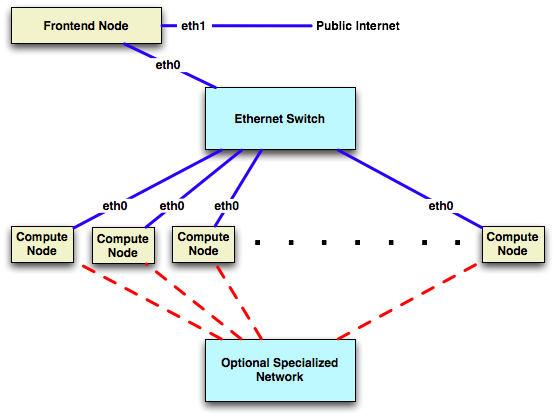
\includegraphics[scale=.5]{cluster.png} 
\paragraph{}
On the Compute nodes (Vm-container), the Ethernet interface that Linux maps to eth0 should be connected to the cluster's Ethernet switch. This network is considered private, i.e, all traffic on this network is physically separated from the external public network (e.g., The Internet).
On the Frontend, at least two Ethernet interfaces are required. The interface that Linux maps to eth0 should be connected to the same Ethernet network as the compute nodes. The interface that Linux maps to eth1 should be connected to the external network (Internet or your organization's intranet).
\paragraph{}
In our case the eth0 is connected to the switch placed within the rack and eth1 of the Frontend is connected to public network under Networks systems lab’s subnet.

\section{Frontend Installation}
The installation on the Frontend is done using a disk image either by a DVD or a bootable USB drive.The Jumbo DVD has all the required rolls in one single disk image. The x86 64 version of Rocks 6.1 can be downloaded from here \cite{rocksdownload}

\begin{itemize}
\item Insert the DVD/USB Drive and restart the main node (Frontend). A boot screen will be displayed with a prompt. Enter the following command to start the installation: 
 \item The next screen shows the list of all rolls in the DVD. Select the required rolls from the list. The Kernel, Base, OS and Web-Server rolls are mandatory. Additional rolls can be installed by using DVD based rolls. Hit next to proceed.
\item The next screen is for entering Cluster Information. Enter the details for Host name, cluster name, organization, locality, state, country, contact, URL, latitude and longitude. The fully-qualified host name is mandatory and is important for several cluster services.
 \item The next screen has the option to set the eth1 ( which is the interface to public network ) IP address. This is the public IP of the cluster(connected to the internet). Enter the public IP as 192.168.41.203.
 
\item The next screen has the option to set the private network eth0 IP address and netmask. This is the IP address of the private network between the Frontend and the nodes. The IP address used is 10.1.1.1 and the netmask is 255.255.0.0.

\item Now configure the gateway and DNS. Gateway used is 192.168.41.1 and DNS servers used are 192.168.254.2, 192.168.254.3.

\item Enter the root password of the cluster when prompted.
\item Configure the time by selecting the time zone for the cluster followed by inputting a Network Time Protocol(NTP) server that will keep the clock on the frontend in sync.

\item The next screen shows the option for the partitioning of the hard disk of the Frontend. Select "Manual Partitioning" since the configuration of " Auto Partitioning provides insufficient space for the /var partition which is used by the Eucalyptus Cloud to upload Virtual Machine Images.

\item The partition used for frontend is: \\ 
\end{itemize}

\begin{center}
\begin{tabular}{ | l | c | r |}
    \hline
    Partition Name & Size  \\ \hline
    /&170GB \\ 
    /var&480GB \\
	/export&170GB \\
	swap&1GB    \\
    \hline
  \end{tabular}
\end{center}


%%%%%%%%%%%%%%%%%%%%%% END OF CHAPTER ONE %%%%%%%%%%%%%%%%%%%%%%%%%%%%%%%%%%%%%%%

%%%%%%%%%%%%%%%%%%%%%% CHAPTER THREE %%%%%%%%%%%%%%%%%%%%%%%%%%%%%%%%%%%%%%%
%%%%%%%%%%%%%%%%%%%%%% CHAPTER Three %%%%%%%%%%%%%%%%%%%%%%%%%%%%%%%%%%%%%%%

\chapter{Network Configuration}

\section{Introduction}
This is the most intriguing part of cloud installation, where we will have to decide upon a networking mode available in Eucalyptus. For Zeus cloud we are using Managed (No VLAN) Mode. Read more about managed no vlan here\cite{managednovlan}.

\subsection{Enabling Public Web Access to Your Frontend}

To permanently enable selected web access to the cluster from other machines on the public network, follow the steps below. Apache's access control directives will provide protection for the most sensitive parts of the cluster web site, however some effort will be necessary to make effective use of them.

To open port 80 (the 'www' service) for the public network of frontend,  execute:

\begin{lstlisting}[language=bash]
rocks open host firewall localhost \
network=public protocol=tcp service=www
\end{lstlisting}
Now you can try accessing the ip \url{192.168.41.203} or uri \url{zeus.nitc.ac.in}over network to view the rocks cluster web frontend.

\subsection{Configuring Firewall}

Eucalyptus components use a variety of ports to communicate. The following table lists the all of the important ports used by Eucalyptus.

\begin{center}
\begin{tabular}{ | l | c | r |}
    \hline
Port&Description \\
TCP 8443& SSL port for the administrative web user interface. Configurable with euca-modify-property.\\
TCP 8772&DEBUG ONLY\\: JMX port. This is disabled by default, and can be enabled with the \-\-debug or \-\-jmx options for CLOUD\_OPTS. \\
TCP 8773&Web services port for the CLC, Walrus, SC, and VB; also used for external and internal communications by the CLC and Walrus. Configurable with euca-modify-property.\\
TCP 8774&Web services port on the CC. Configured in the eucalyptus.conf configuration file.\\
TCP 8775&Web services port on the NC. Configured in the eucalyptus.conf configuration file.\\
TCP 8776&Used by the image cacher on the CC. Configured in the eucalyptus.conf configuration file.\\
TCP 8777&Database port on the CLC.\\
TCP 8080&Port for the administrative web user interface. Forwards to 8443. Configurable with euca-modify-property.\\
UDP 7500&Distributed cache port on the CLC, Walrus, SC, and VB.\\
UDP 8773&HA membership port.\\
TCP/UDP 53&DNS port on the CLC.\\
\end{tabular}
\end{center}

\subsection{To open the required ports,run the following commands}
Here we are trying to open ports for Eucalyptus to communicate between its components, rocks command \emph{rocks add firewall} can be used to add firewall rules. 

Read the following rocks manual to understand more Managing firewall through Rocks \cite{mfirewal}.

\subsection{Opening ports in Frontend}
\begin{lstlisting}[language=bash]
rocks add firewall host=frontend network=public protocol=tcp service=8443 \ chain=INPUT action=ACCEPT rulename=E10-PORT-8443

rocks add firewall host=frontend network=public protocol=tcp service=8772 \
chain=INPUT action=ACCEPT rulename=E10-PORT-8772

rocks add firewall host=frontend network=public protocol=tcp service=8773 \
 chain=INPUT action=ACCEPT rulename=E10-PORT-8773

rocks add firewall host=frontend network=public protocol=tcp service=8774 \ 
chain=INPUT action=ACCEPT rulename=E10-PORT-8774

rocks add firewall host=frontend network=public protocol=tcp service=8776 \ 
chain=INPUT action=ACCEPT rulename=E10-PORT-8776

rocks add firewall host=frontend network=public protocol=tcp service=8777 \ 
chain=INPUT action=ACCEPT rulename=E10-PORT-8777

rocks add firewall host=frontend network=public protocol=tcp service=8080 \
chain=INPUT action=ACCEPT rulename=E10-PORT-8080

rocks add firewall host=frontend network=public protocol=tcp service=5005 \
chain=INPUT action=ACCEPT rulename=E10-PORT-5005

rocks add firewall host=frontend network=public protocol=udp service=7500 \
chain=INPUT action=ACCEPT rulename=E10-PORT-7500
\end{lstlisting}


Before synchronising the firewall rules we need to remove two rules from the existing firewall.
The command to remove the rules are 
\begin{lstlisting}[language=bash]
rocks remove firewall global rulename=R900-PRIVILEGED-TCP
rocks remove firewall global rulename=R900-PRIVILEGED-UDP
\end{lstlisting}
\subsection{Opening Web Access to Public}
Remove the rule which restrict the web access only to subnet 192.168.41.0/24
\begin{lstlisting}[language=bash]
rocks remove firewall host=localhost rulename=A40-WWW-PUBLIC-LAN
\end{lstlisting}

\subsection{Now, make it available to public}
\begin{lstlisting}[language=bash]
rocks add firewall host=frontend network=public protocol=tcp \
service=www chain=INPUT action=ACCEPT \
flags="-m state --state NEW --source 0.0.0.0/0.0.0.0" \
rulename=A40-WWW-PUBLIC-NEW
\end{lstlisting}
\subsection{Sync the above firewall rules to rocks frontend using }
\begin{lstlisting}[language=bash]
rocks sync host firewall frontend
\end{lstlisting}
\subsection{Accepting everything from TCP and UDP }
\begin{lstlisting}[language=bash]
iptables -A INPUT -p udp --dport 0:1023 -j ACCEPT
iptables -A INPUT -p tcp --dport 0:1023 -j ACCEPT
/sbin/service iptables save
\end{lstlisting}
\subsection{Opening ports required for DNS functioning}

\begin{lstlisting}[language=bash]
iptables -A INPUT -p tcp -m tcp --sport 53 --dport 1024:65535 -m state \ --state ESTABLISHED -j ACCEPT
iptables -A INPUT -p udp -m udp --sport 53 --dport 1024:65535 -m state \ --state ESTABLISHED -j ACCEPT
iptables -A OUTPUT -p tcp -m tcp --sport 1024:65535 --dport 53 -m state \ --state NEW,ESTABLISHED -j ACCEPT
iptables -A OUTPUT -p udp -m udp --sport 1024:65535 --dport 53 -m state \ --state NEW,ESTABLISHED -j ACCEPT
/sbin/service iptables save

\end{lstlisting}
\subsection{Opening ports in nodes}
Opening the web service in nodes
\begin{lstlisting}[language=bash]
rocks add firewall appliance=vm-container protocol=tcp \
service=8775 network=all chain=INPUT action=ACCEPT \
rulename=E10-PORT-8775
\end{lstlisting}
\subsection{Sync the firewall rules to all the nodes using }
\begin{lstlisting}[language=bash]
rocks sync host firewall vm-container
\end{lstlisting}
\section{Verify TCP/IP Connectivity}

Verify connectivity between the machines you’ll be installing Eucalyptus on. Some Linux distributions provide default TCP/IP firewalling rules that limit network access to machines. Disable these default firewall settings before you install Eucalyptus components to ensure that the components can communicate with one another.
Verify component connectivity by performing the following checks on the machines that will be running the listed Eucalyptus components.
\begin{enumerate}
\item Verify connection from and end-user to the CLC on ports 8773 and 8443
\item Verify connection from an end-user to Walrus on port 8773
\item Verify connection from the CLC, SC, and NC to Walrus on port 8773
\item Verify connection from Walrus, SC, and VB to CLC on port 8777
\item Verify connection from CLC to CC on port 8774
\item Verify connection from CC to VB on port 8773
\item Verify connection from CC to NC on port 8775
\item Verify connection from NC (or VB) to Walrus on port 8773 or you can verify the connection from the CC to Walrus on port 8773, and from an NC to the CC on port 8776
\item Verify connection from public IP addresses of Eucalyptus instances (metadata) and CC to CLC on port 8773
\item Verify TCP connectivity between CLC, Walrus, SC and VB
\item Verify connection between CLC, Walrus, SC, and VB on UDP ports 7500 and 8773

\end{enumerate}
We will use the program given below as socket which will  listen to specified a port (as a server ), run this program and telnet to the server's ip ( where you ran the program ) along with port number and check the connection.

\begin{lstlisting}[language=java]
import java.net.*;
import java.io.*;
public class PortMonitor {
    public static void main(String[] args) throws Exception {
         //Port to monitor
        final int myPort = Integer.parseInt(args[0]);
        ServerSocket ssock = new ServerSocket(myPort);
        System.out.println("port " + myPort + " opened");
         Socket sock = ssock.accept();
        System.out.println("Someone has made socket connection");
         OneConnection client = new OneConnection(sock);
        String s = client.getRequest();
     }
 }
class OneConnection {
    Socket sock;
    BufferedReader in = null;
    DataOutputStream out = null;
OneConnection(Socket sock) throws Exception {
        this.sock = sock;
        in = new BufferedReader(new InputStreamReader(sock.getInputStream()));
        out = new DataOutputStream(sock.getOutputStream());
    }
String getRequest() throws Exception {
        String s = null;
        while ((s = in.readLine()) != null) {
            System.out.println("got: " + s);
        }
        return s;
    }
}
\end{lstlisting}
Example 
( 1 ) Verify connection from and end-user to the CLC on ports 8773

Now run the program in frontend with argument 8773
\begin{lstlisting}[language=bash]
javac Portmonitor.java
java Portmonitor 8773
\end{lstlisting}
From any other system telnet into frontend with port 8773
\begin{lstlisting}[language=bash]
telnet 192.168.41.203 8773
Trying 192.168.41.203...
Connected to 192.168.41.203.
Escape character is '^]'.
hello
\end{lstlisting}
Output @ frontend when connection is established 
\begin{lstlisting}[language=bash]
port 8773 opened
Someone has made socket connection
got: hello
\end{lstlisting}
Understand the scenario for each of the verification step given above using the program and telnet.

\section{Configure SELinux}
SELinux is not supported by Eucalyptus
\begin{enumerate}
\item Open /etc/selinux/config and edit the line SELINUX=enforcing to SELINUX=permissive.
\item Save the file.
\item Run the following command: \\
\em{setenforce 0}
\end{enumerate}
\section{Configure NTP}

Eucalyptus requires that each machine have the Network Time Protocol (NTP) daemon started and configured to run automatically on reboot.
\linebreak
NTP in Frontend
\linebreak
Check the status of ntpd daemon 
\em{service ntpd status}
\linebreak
Update the time using any server
\em{ntpdate -u 0.pool.ntp.org}
\linebreak
Sync the time with the hardware clock 
\em{hwclock --systohc}
\linebreak
NTP in Nodes
\em{rocks run host vm-container “ntpd -u 0.pool.ntp.org ; hwclock --systohc”}

%%%%%%%%%%%%%%%%%%%%%% END OF CHAPTER THREE %%%%%%%%%%%%%%%%%%%%%%%%%%%%%%%%%%
%%%%%%%%%%%%%%%%%%%%%%%%%%% END OF CHAPTER THREE %%%%%%%%%%%%%%%%%%%%%%%%%%%%%%%%%%%%%%%